\section{Laboratory work implementation}

\subsection{Tasks and Points}

- Realizeaza un simplu site; \\
\indent 
- Site-ul trebuie sa contina AJAX Requests; \\
\indent 
- Implimentarea XHR sau JSON responses. Careva din informatie trebuie sa fie dinamic incarcata pe pagina;

\subsection{Analiza lucrarii de laborator}
\selectlanguage{russian}
В ходе данной лабораторной работы был разработан сайт, содержащий информацию о лабораторных работах со второй по пятую. Сайт состоит из двух страниц. На первой происходит авторизация или регестрация. На второй присутствует счетчик, который позволяет выбрать номер необходимой лабораторной работы. Информация загружается на страницу динамически с помощью технологии AJAX.\\
\indent 
Созданный сайт имеет связь с базой данных. Используется база данных MySql. При этом было создано две отдельные базы. Одна содержит таблицу с логинами и паролями. Вторая база данных содержит информацию о лабораторных работах. Для каждой из них создана отдельная таблица. Для каждого из подпунктов используется отдельный столбец.(рис.1)\\
\indent 
Для обеспечения функциональности использовались технологии и языки PHP, HTML, CSS и JavaScript. На языке HTML написаны сами страницы. При этом присутствует только один файл index.html. Разметка для второго файла отправляется вместе с файлом main2.php. В файлах .php находятся команды, которые позволяют взаимодействовать с базой данных. Чтобы обратиться к какому либо из файлов на сервере, мы отправляет запрос по адресу http://localhost/name/nameOfFile. В лабораторной работе используются только один тип запросов - POST. При регестрации в теле запроса отправляются логин и пароль в обычном текстовом формате. \\
\indent 
При AJAX запросах, данные на сервер и с сервера отправляются в формате JSON. На сервере этот формат обрабатывается с помощью специальных функций. Но при установки моей версии PHP библиотека по работе с JSON установлена не была, поэтому на сервере присутствует дополнительная библиотека, из которой берутся функции для работы с JSON на сервере. Сам запрос и генерация JSON прописаны в файле RequestsAjax.js. В этом же файле парсится и распределяются данные из полученного с сервера ответа.\\
\indent 
Коды можно просмотреть на репозитории 



\subsection{Imagini}

\begin{figure}[h]
	\center{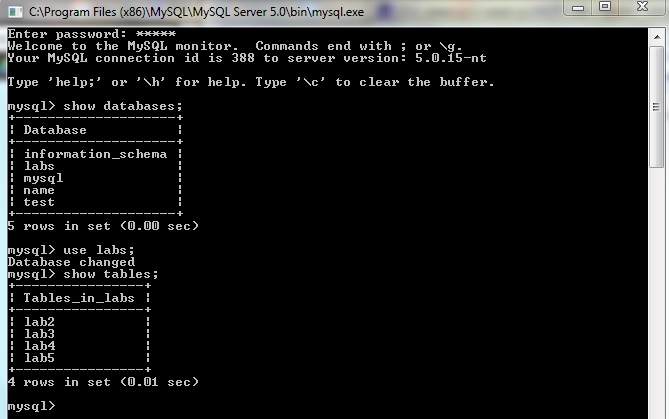
\includegraphics[width=1\linewidth]{images/DB.jpg}}
	\caption{База данных}
	\label{ris:image}
\end{figure}
\hfill
\begin{figure}[h]
	\center{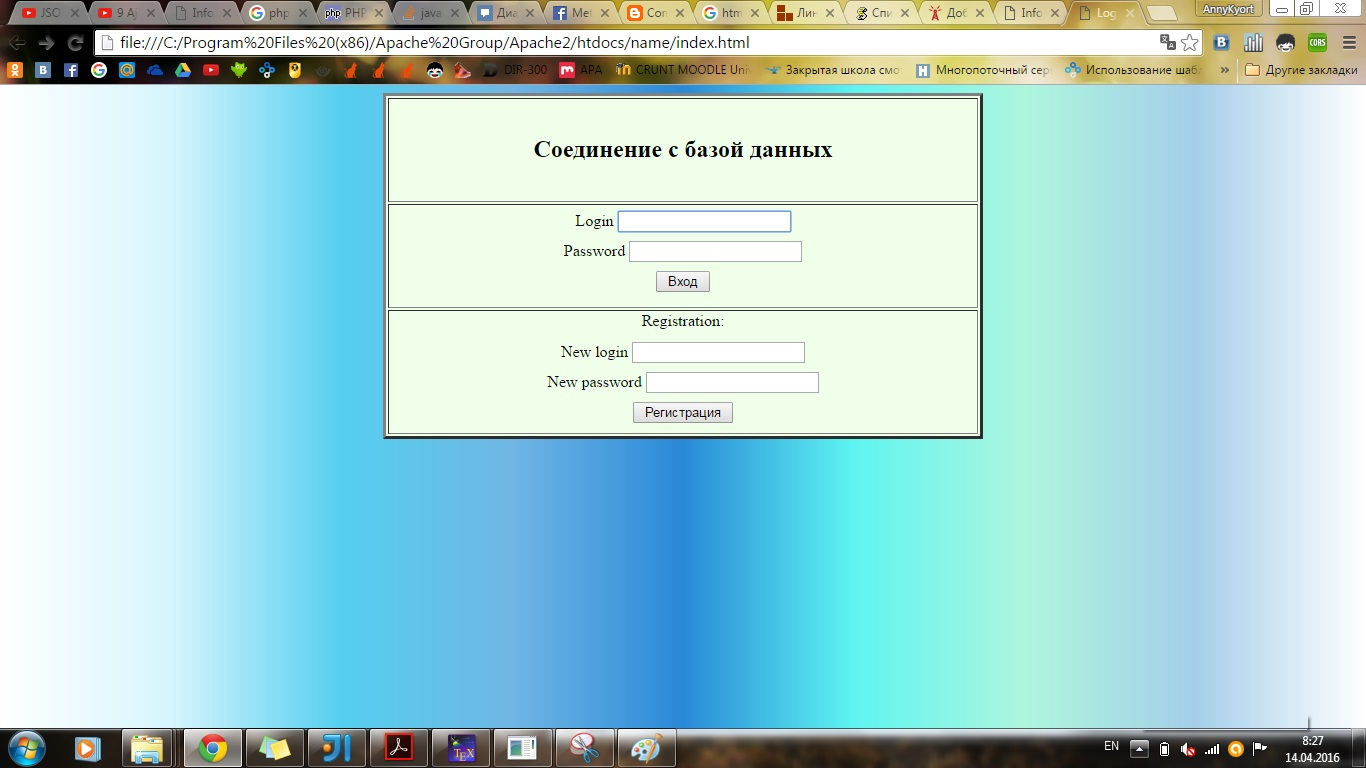
\includegraphics[width=1\linewidth]{images/Regestr.jpg}}
	\caption{Страница регестрации}
	\label{ris:image}
\end{figure}
\hfill
\begin{figure}[h]
	\center{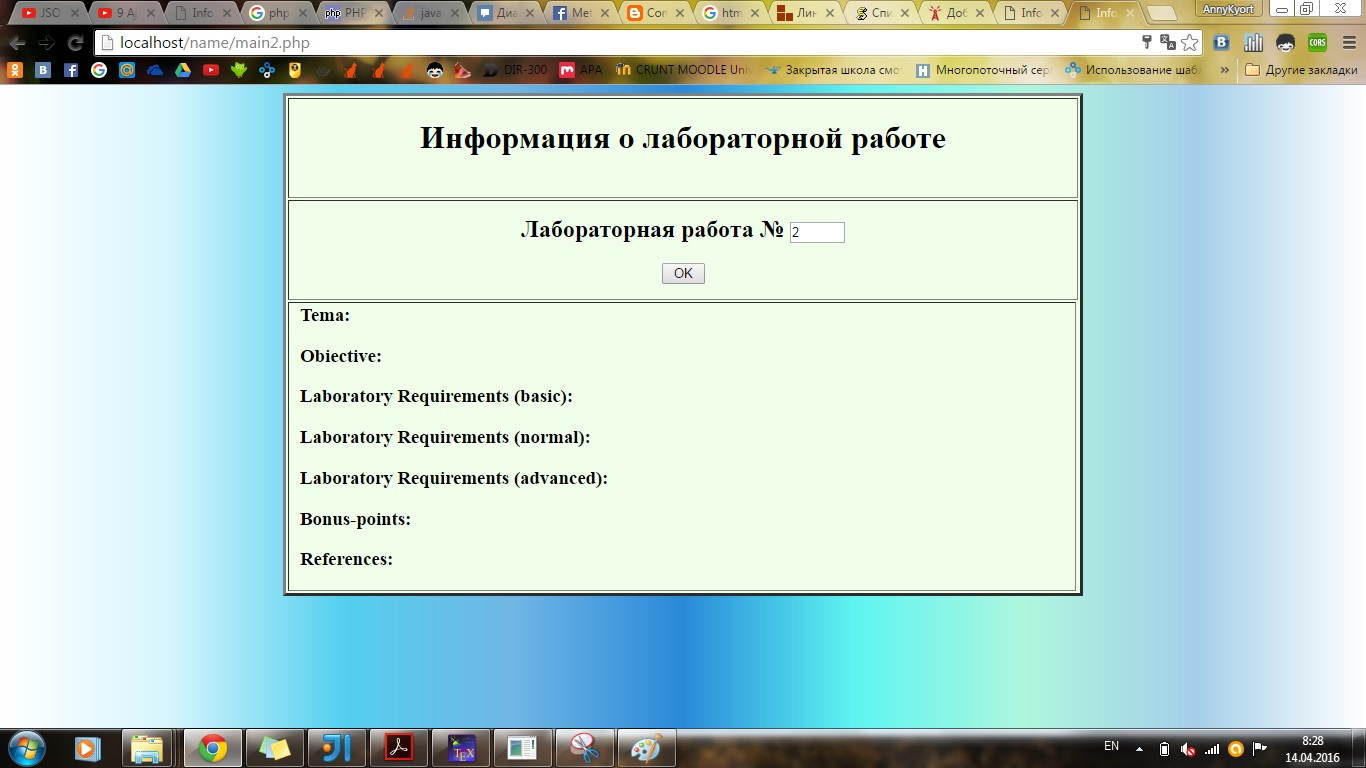
\includegraphics[width=1\linewidth]{images/Main1.jpg}}
	\caption{Основная страница без данных}
	\label{ris:image}
\end{figure}
\hfill
\begin{figure}[h]
	\center{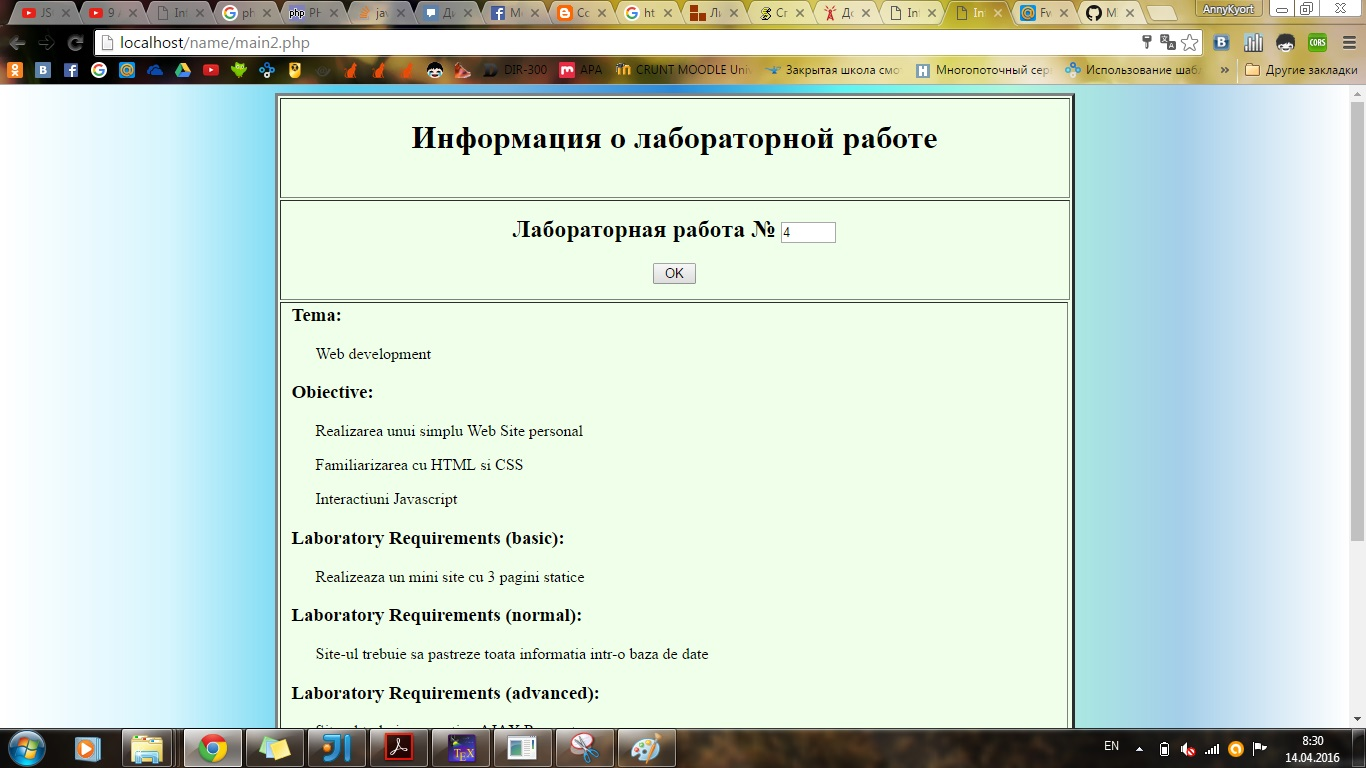
\includegraphics[width=1\linewidth]{images/Main2.jpg}}
	\caption{Основная страница с данными}
	\label{ris:image}
\end{figure}

\clearpage